\documentclass[12pt]{article}

% The geometry package allows for easy page formatting.
\usepackage[margin=20mm]{geometry}
\geometry{letterpaper}

% Load up special logo commands.
\usepackage{doc}

% Package for formatting URLs.
\usepackage{url}

\usepackage{braket}
\usepackage{bbold}
\usepackage{amsmath, amsfonts, amsthm}
\usepackage{amssymb}
\usepackage{pgfplots}
\usepackage{mathtools}

\usepackage{multicol}
\usepackage{wrapfig}
\usepackage{subfig}

% Packages and definitions for graphics files.
\usepackage{graphicx}
\graphicspath{ {./figures/} }		% path of images

\usepackage{epstopdf}
\DeclareGraphicsRule{.tif}{png}{.png}{`convert #1 `dirname #1`/`basename #1 .tif`.png}

%
% Set the title, author, and date.
%
\title{A Study on Star Clusters}
\author{Anthony Karoki Mugambi$^{1, 2}$\\
	\small $^1$I44/1899/2018\\
	\small $^2$Department of Physics, University of Nairobi, Chiromo Campus, Nairobi, Kenya
}
\date{}

%
% Instantiate commands
%

\renewcommand{\thefootnote}{\fnsymbol{footnote}}  %use symbolic footnote

%
% Keywords command
\providecommand{\keywords}[1]
{
	\small	
	\textbf{\text{Keywords: }} #1
}


%
% The document proper.
%
\begin{document}
	\maketitle
	
	\begin{abstract}
		We take on a study if two types of star clusters to determine their age and distances. Using collected data, we will show how clusters can be used to measure the relative distances and ages of stars in the cluster. Optical and infrared data will be used to generate a CMD graph. In this exercise, you will determine the colour of many cluster members and plot them on a Colour-Magnitude diagram.%This is just a type of Hertzsprung-Russell (HR) diagram in which we plot Colour Index rather than Spectral Class on the horizontal axis; and use the apparent visual magnitude, V, for the vertical axis.
	\end{abstract}

	\keywords{colour-magnitude diagrams, globular clusters, open clusters}
	
	\pagebreak
	\tableofcontents
	
	\pagebreak
	\listoffigures

	\pagebreak
	\section{Introduction}
	\label{sec:intro}
	Most stars in the universe form in clusters. Star clusters are group of stars that share a common origin and are gravitationally bound together hence move collectively since their stellar motions are completely correlated and not random. The star clusters are formed at the same time and from the same gas cloud, and they thus have similar age and are found at a common distance as viewed from Earth. The common age and distance makes stellar clusters particularly important in studies and models of stellar evolution, stellar ages and luminosities. For this reason, photometric measurements can be used to determine the age of a cluster and its distance as viewed from Earth.\\
	The two basic categories of stellar clusters are open clusters and globular clusters.\\
		\subsection{Open Cluster}
		Open clusters are diffuse star clusters hosting a few hundreds or thousands of stars. Individual component stars are easily resolved with telescopes hence the name open cluster. They are mostly found on the dusty spiral arms on the plane of spiral galaxies.\\
		In this paper, we shall look at the open cluster Messier 7 (M7) or NGC 6475.
		\subsection{Globular Cluster}
		Globular clusters are spheroidal collections of several hundred thousands to a million stars found orbiting in the halos of all large galaxies. They tend to be very densely packed, hosting millions of stars in the space of only a few parsecs. They comprise the oldest stars in the galaxy.\\
		In this paper, we shall look at the globular cluster Messier 54 (M54) or NGC 6715.
		\subsection{Importance of Stellar Clusters}
		The main motivation of studying stellar clusters is because they allow astronomers to improve on current the current model and knowledge bank of stellar evolution and ages of stars. By fact that this stars arose from the same molecular gas cloud, member stars in the cluster share effectively the same evolutionary trajectory.\\
		Also, the member stars are effectively at the same distance from an observer on Earth. We say this and more so why this is logically true is because the distance from the cluster to Earth is significantly greater than the distances among the stars spatially distributed within the cluster.\\
		The relevant photometric measurement needed is the apparent magnitude of member stars of the cluster. Such data helps to infer the relative absolute magnitudes of stars in the cluster. This is relevant in the creation of a colour-magnitude diagram (CMD) for a specific cluster. The CMD is a HR graph that plots apparent magnitude, V, on the vertical axis against colour index (CI$^1$) on the horizontal axis.\\
		Colour index is a simple numerical expression the determines the colour of an object. An object's luminosity is observed through two different filters, e.g. B and V (blue light and green-yellow visible light). The difference in the luminosities, i.e. B - V, is the colour index. A smaller colour index indicates a bluer hence hotter star while a larger colour index indicates a redder/cooler star.
		\footnote{CI = B - V}
	
	
	
	\pagebreak
	\section{Theory and Background Information}
	Our clusters of study are the M7 open cluster and M54 globular cluster.
		\subsection{Terminology}
		Apparent magnitude is a logarithmic measurement of the brightness of stars/celestial objects as viewed from Earth. It is based on how human eyes view different levels of brightness. It is denoted by \textbf{m} and measured in magnitudes.\\
		Absolute magnitude is a measurement of a star's/celestial object's brightness if it were located at a distance of 10 parsecs. It is a measure of the true brightness. It is denoted by \textbf{M} and measured in magnitudes.
		\subsection{Messier 7 Open Cluster}
		\begin{wrapfigure}{l}{0.6\textwidth}
			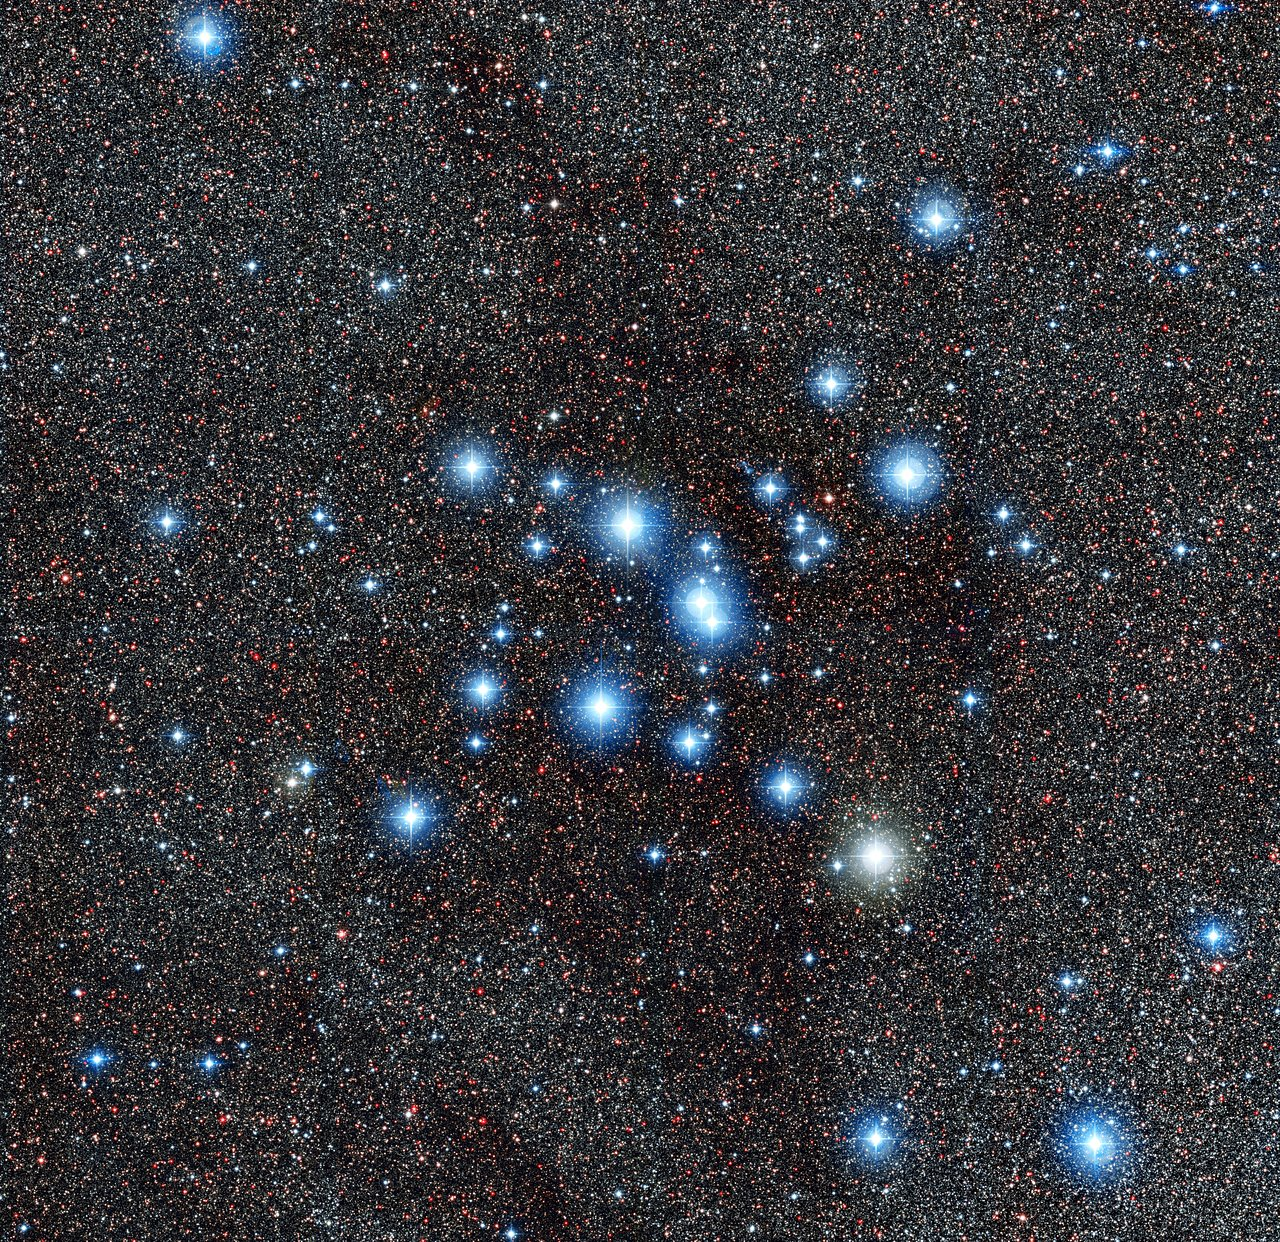
\includegraphics[width=0.58\textwidth]{m7_eso_0}
			\caption{This new image from the Wide Field Imager on the MPG/ESO 2.2-metre telescope at ESO’s La Silla Observatory in Chile, shows the bright star cluster Messier 7, also known as NGC 6475. Easily spotted by the naked eye in the direction of the tail of the constellation of Scorpius (The Scorpion), this cluster is one of the most prominent open clusters of stars in the sky and an important research target. \cite{eso_m7} Credit: ESO}
			\label{fig: m7}
		\end{wrapfigure}
		\textbf{M7} also goes by the designations \textbf{NGC 6475} and \textbf{Ptolemy's Cluster}. M7 was known as early as the year 130 CE when it was mentioned by Claudius Ptolemy, a 2$^{nd}$ century Greek Astronomer and Mathematician. It is a large prominent bright star cluster visible to the naked eye in the constellation Scorpius.\\
		It is part of the Milky Way galaxy. It has an apparent visual magnitude of 4.1 and its angular diameter is 80 arc-minutes making it easy to see with the naked eye. M7 lies at an estimated distance of 800 light years or about 300 parsecs. It's Right Ascension is 17h 53.9m while its Declination is -34° 49´\cite{astropixels_m7}.\\
		Messier 7 contains about 80 stars between magnitudes 6 and 10. It is believed to be about 220 million years old and has a mass about 735 times that of the Sun. It is approaching us at a speed of 14 km/s. The brightest star in the cluster is a yellow G8-type giant with an apparent magnitude of 5.6.\\
		The stars in M7 were all formed at roughly the same time in the same large cosmic cloud and they therefore are an invaluable insight into stellar evolution and structure \cite{messier007}.\\
		\subsection{Messier 54 Globular Cluster}
		\textbf{M54} also goes by the designation \textbf{NGC 6715}. It is a compact globular cluster.\\
		It was the first extragalactic cluster ever discovered and is recognized as part of the Sagittarius Dwarf Galaxy (SDG), a satellite galaxy of the Milky Way\cite{nasa_m54}. It is located in the southern constellation Sagittarius. It has an apparent visual magnitude of 7.6 and its angular diameter is 9.1 arc-minutes. M54 lies at an estimated distance of 88,700 light years. It has a Right Ascension of 18h 55.1m and a Declination of -30° 29´.\\
		The estimated age of M54 is 13 billion years. Current estimates indicate that the M54 cluster, is situated almost 90 000 light-years away. Messier 54 occupies an area of 12 arc minutes, corresponding to a true radius of 153 light years.\\
		It is a quite concentrated and dense globular cluster with an absolute magnitude of -10 and a luminosity about 850,000 times that of the Sun \cite{messier54}.
		\begin{figure}%{l}{0.52\textwidth}
			\centering
			\subfloat[\centering Hubble image of M54. \cite{esahubble_images} Credit: ESA/Hubble $\&$ NASA]{{	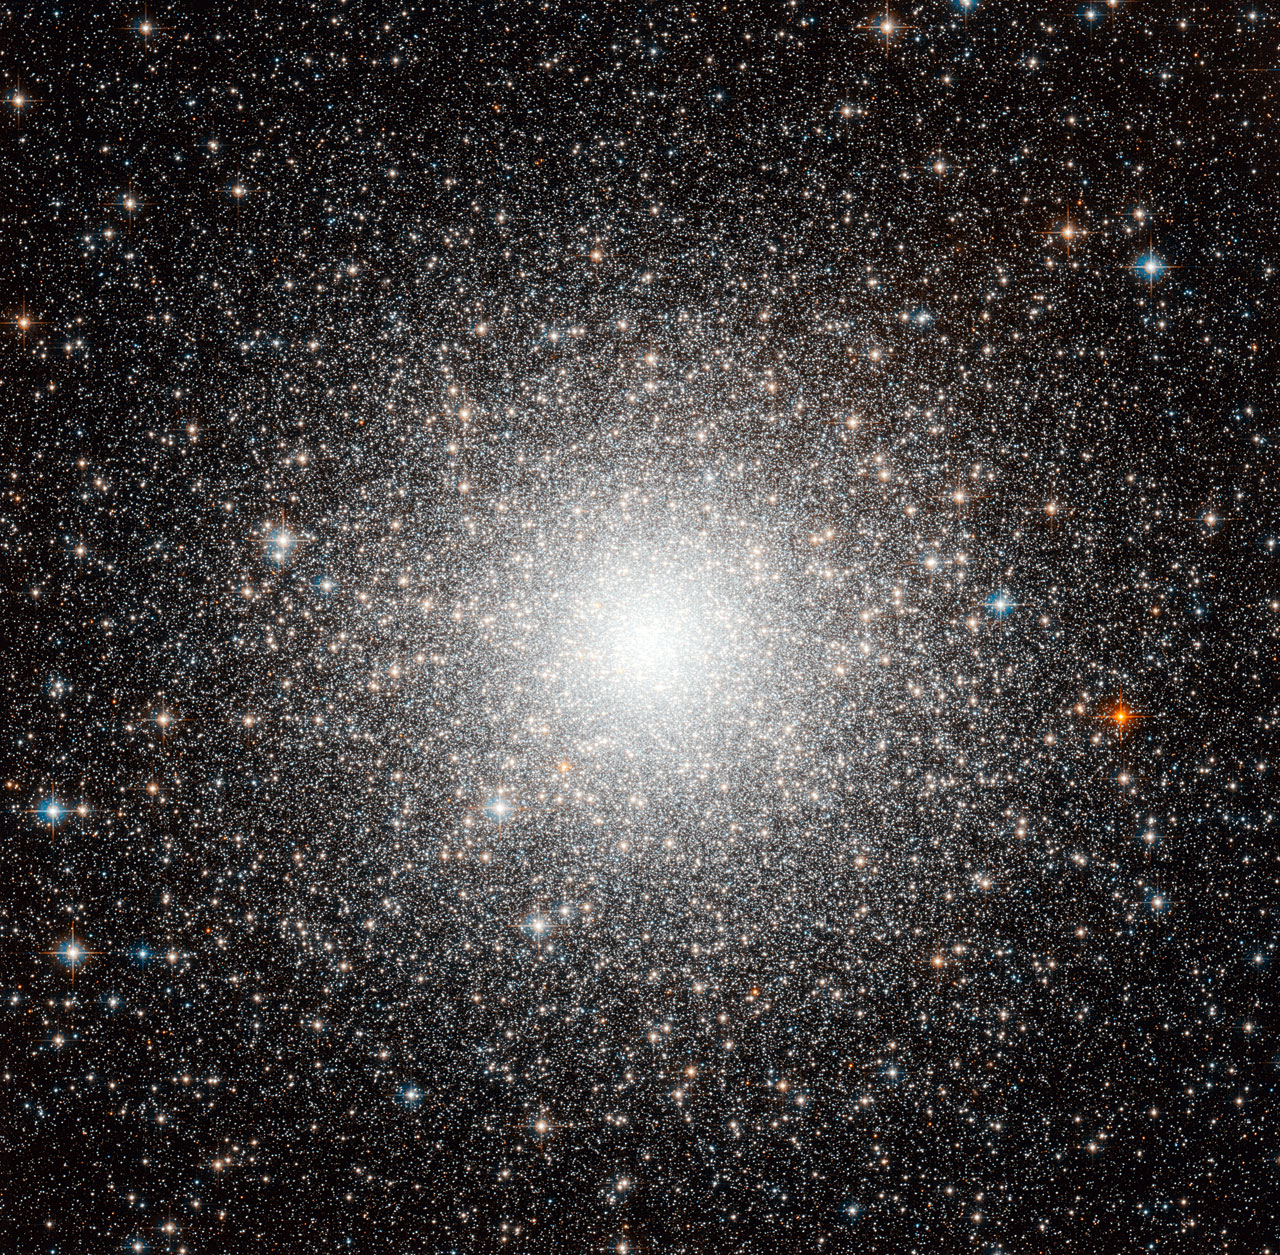
\includegraphics[width=0.5\textwidth, keepaspectratio]{m54_esa_nasa_hubble_0} }}
			%\qquad
			\subfloat[\centering This image from the VLT Survey Telescope at ESO’s Paranal Observatory in northern Chile shows the globular cluster Messier 54. This cluster looks very similar to many others, but it has a secret. Messier 54 doesn’t belong to the Milky Way, but actually is part of a small satellite galaxy, the Sagittarius Dwarf Galaxy. This unusual parentage has allowed astronomers to use the Very Large Telescope (VLT) to test whether unexpectedly low levels of the element lithium in stars are also found in  stars outside the Milky Way. \cite{eso_m54} Credit: ESO]{{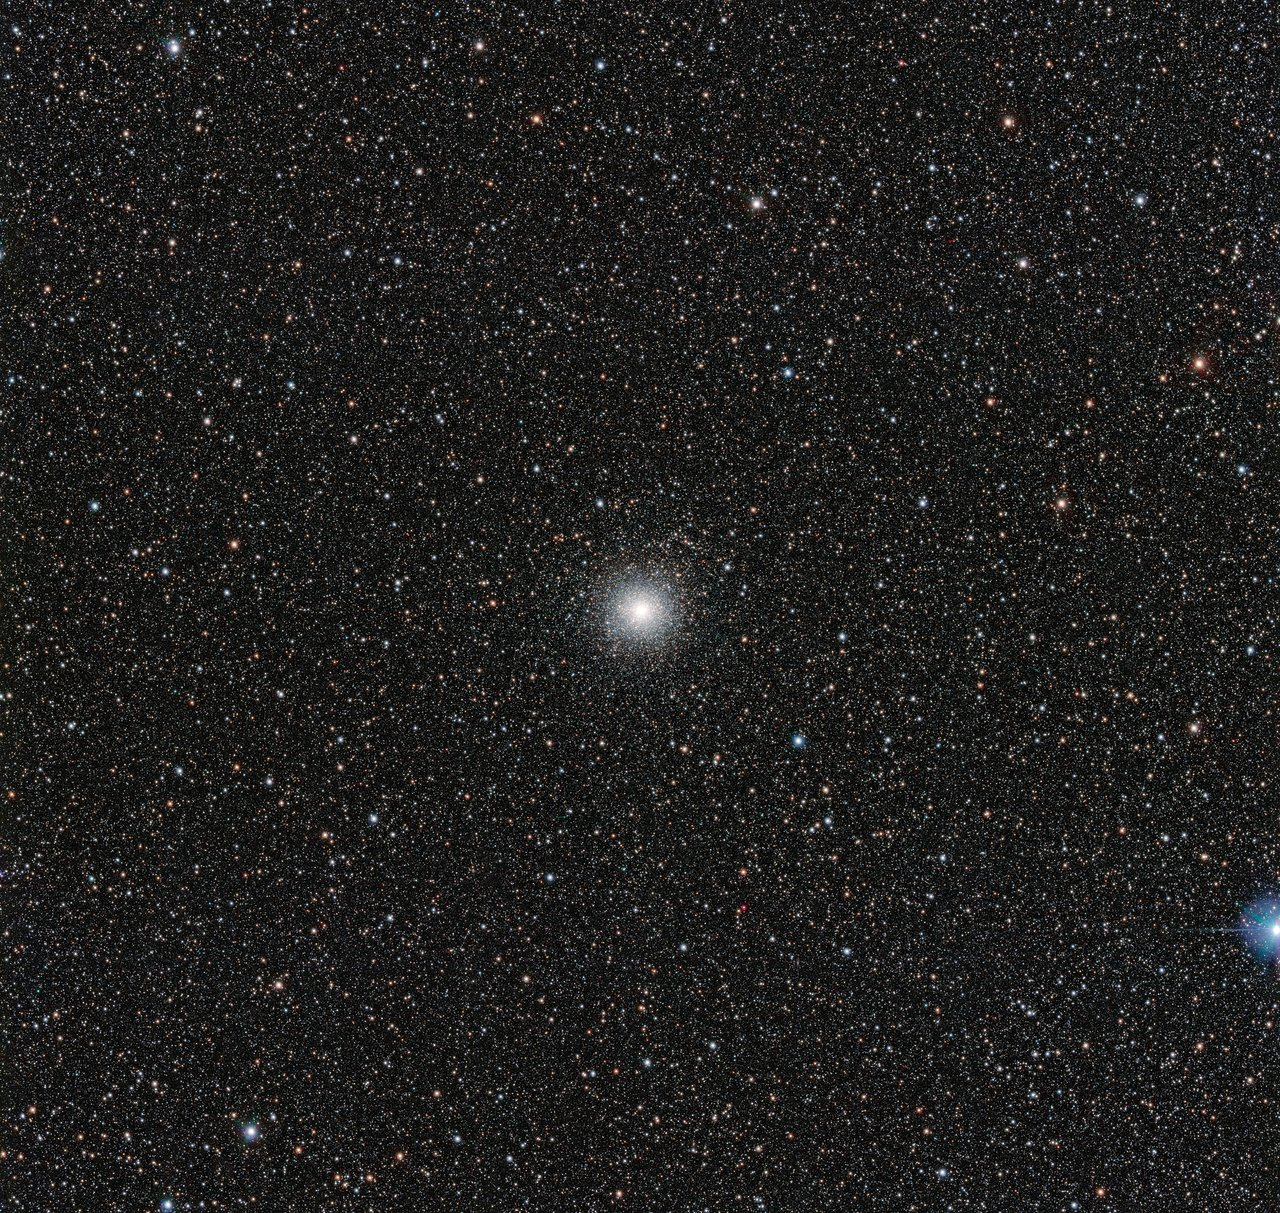
\includegraphics[width=0.5\textwidth, keepaspectratio]{m54_eso_0}}}
			\caption{M54 stellar cluster}
			\label{fig: m54_cluster}
		\end{figure}
%		\begin{figure}[h!]%{l}{0.5\textwidth}
%			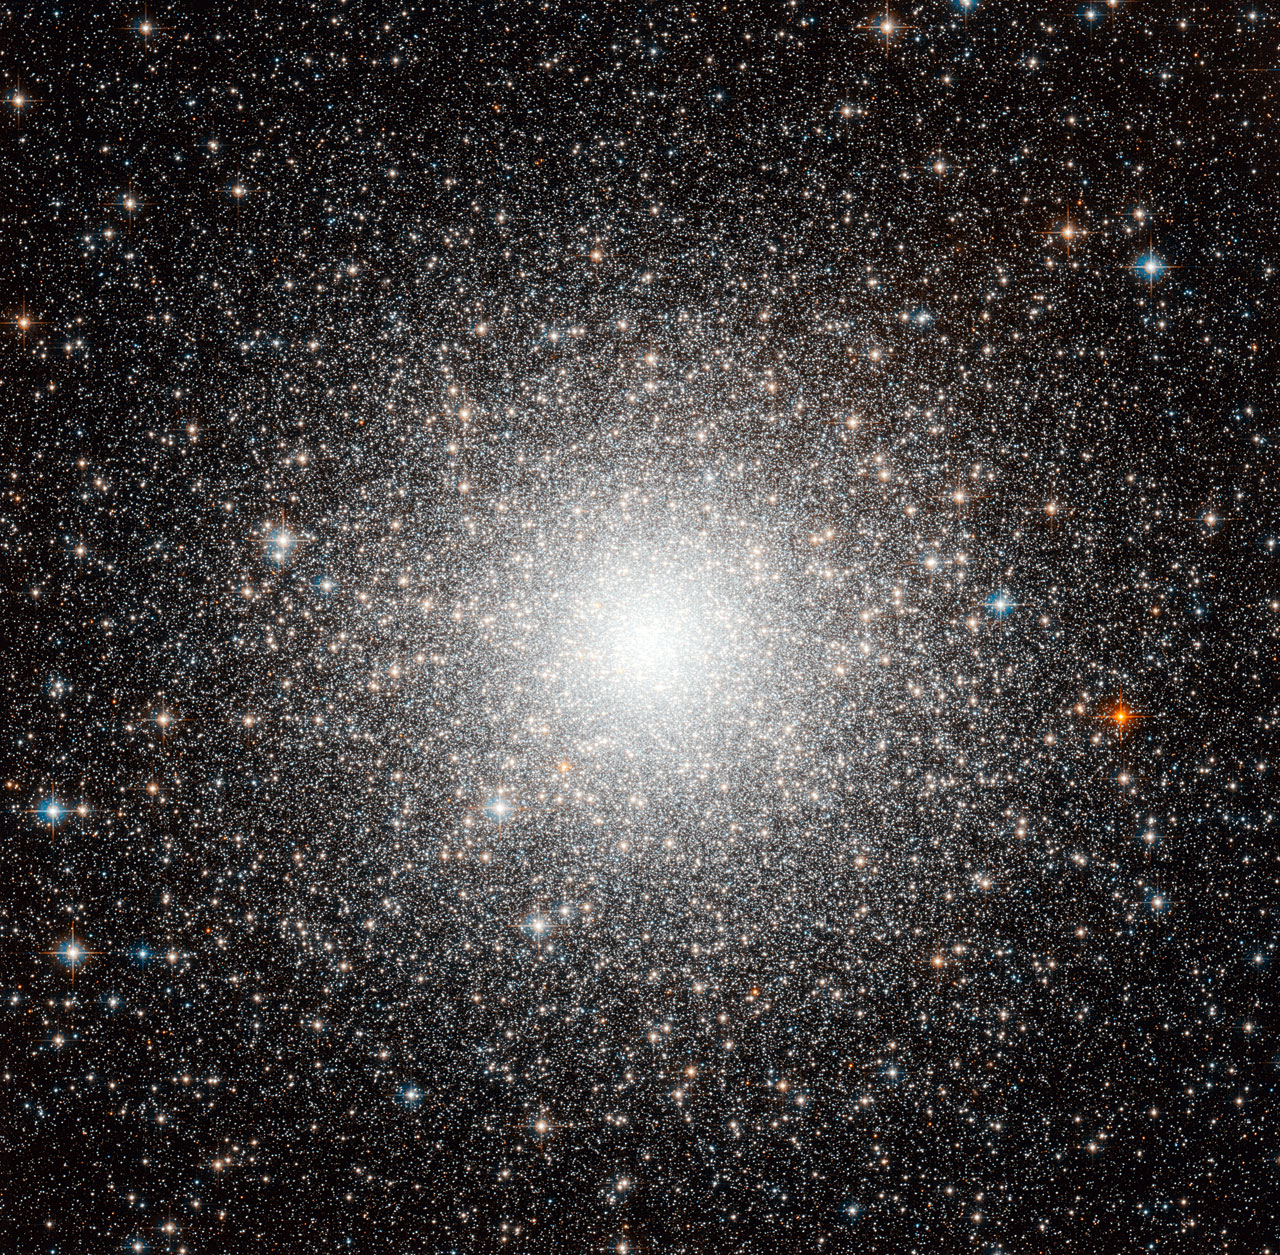
\includegraphics[width=0.5\textwidth]{m54_esa_nasa_hubble_0}
%			\caption{Hubble image of M54. \cite{esahubble_images}\\Credit: ESA/Hubble $\&$ NASA}
%			\label{fig: m54}
%		\end{figure}
%		\begin{figure}[h!]%{r}{0.5\textwidth}
%			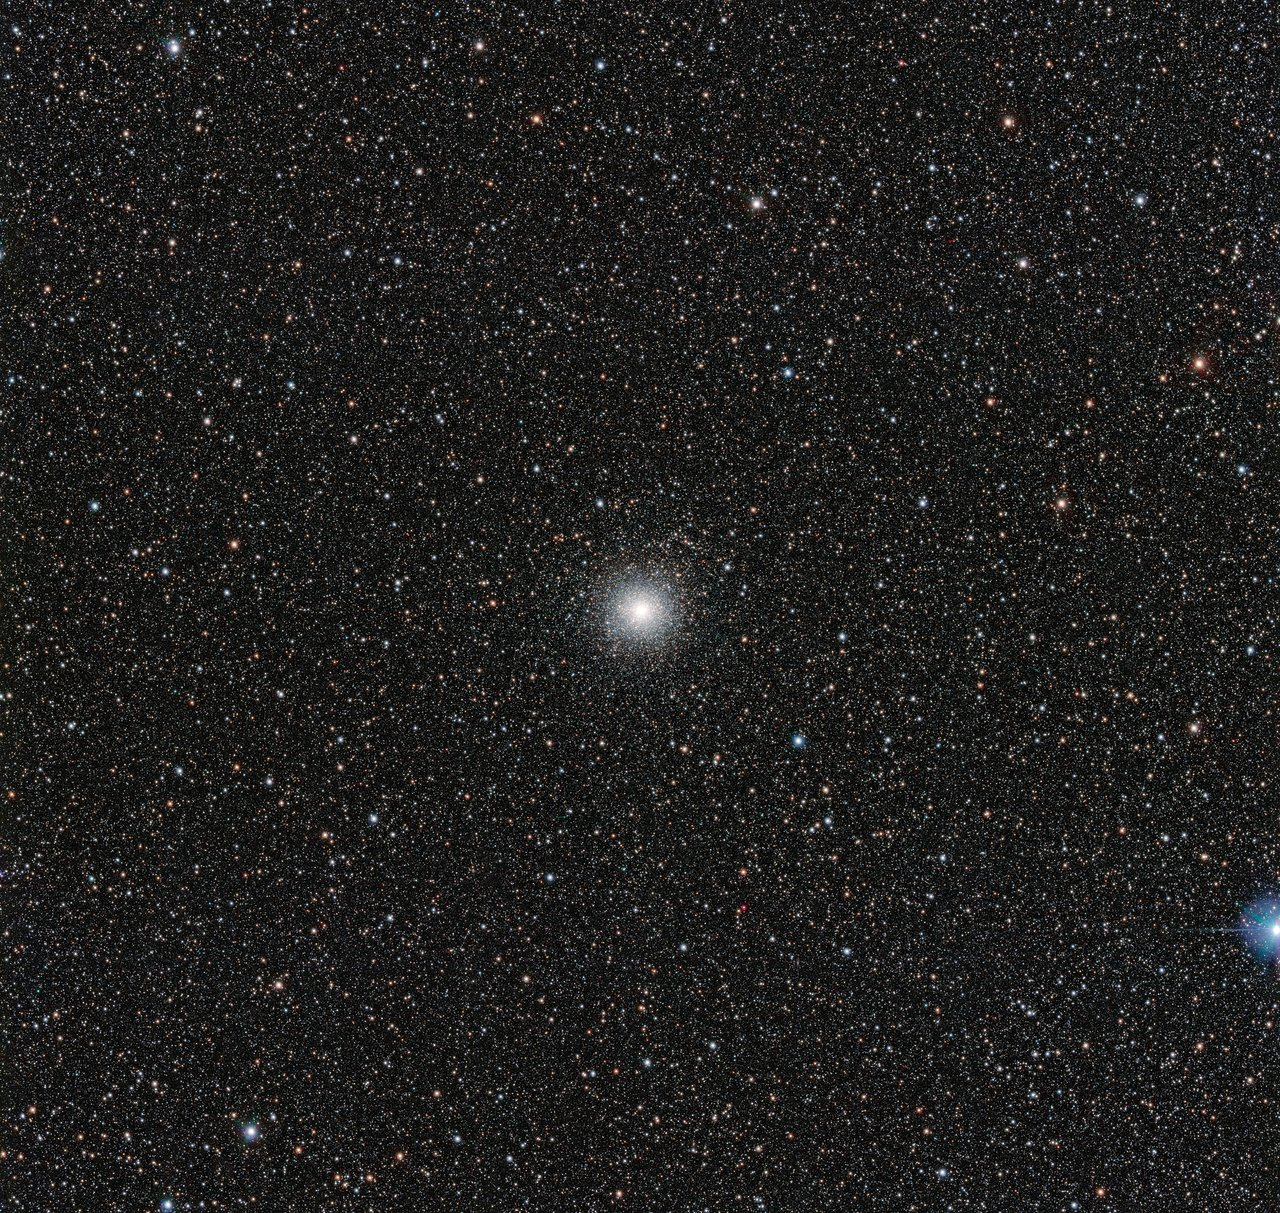
\includegraphics[width=0.5\textwidth]{m54_eso_0}
%			\caption{This image from the VLT Survey Telescope at ESO’s Paranal Observatory in northern Chile shows the globular cluster Messier 54. This cluster looks very similar to many others, but it has a secret. Messier 54 doesn’t belong to the Milky Way, but actually is part of a small satellite galaxy, the Sagittarius Dwarf Galaxy. This unusual parentage has allowed astronomers to use the Very Large Telescope (VLT) to test whether unexpectedly low levels of the element lithium in stars are also found in  stars outside the Milky Way. \cite{eso_m54}\\Credit: ESO}
%			\label{fig: m54_1}
%		\end{figure}
		
		\subsubsection{Data Analysis}
		We will be collecting photometric data and use it to construct a CMD graph for the stars. From this we can derive a star's colour and temperature which is useful in calculating distances to star clusters and estimating the age of a star cluster.\\
		A star's magnitude tells us about its luminosity. On determining a star's absolute magnitude, we can estimate its distance from us. A star's colour also tells us about its surface temperature.\\
		Normally, the methodology or procedure to follow is; plotting the visual magnitudes, V, of stars against their B-V colour indices. This will result in a graph that resembles a HR diagram.\\
		In our case, we are using infrared data. Our images are 3-band composites constructed from 2MASS Atlas images. The infrared images are then mapped into false colours. The 3 bands are named J, H and K.\\
		The J band is taken at a wavelength of $1.235\mu m$ and mapped into the false colour blue. The H band is taken at a wavelength of $1.662\mu m$ and mapped into the false colour green. The K band is taken at a wavelength of $2.159\mu m$ and is mapped into the false colour red.\\
		
	
	
	\section{Methodology and Procedure}
	We have determined that photometric measurements can be used to determine the age and distances of clusters. By taking photometric images of our clusters through separate colour filters. Since we eill be using the 2MASS infrared images, we will make use of the J and K band filters, to measure the apparent magnitude of each star in each waveband colour. Our colour index CI is going to be given by $CI = J - K$.\\
	Our method of finding a star's brightness, among the many that exists, is aperture photometry.
		\subsection{Database}
		To get the data for the star clusters M7 and M54, we use the data archives from NASA/IPAC EXTRAGALACTIC DATABASE (NED) website. For each star cluster, the infrared data is found at the NASA/IPAC Infrared Science Archive page of the NED website. We get 2MASS Interactive Image Service Results where we download the J, K and H bands of the 2MASS Atlas images.
		\subsection{Software and Tools}
		Other than the relevant websites where data is downloaded, we also make use of various software programs to manipulate, analyze and make sense of the data collected.\\
		For this study these tools are; SAOImageDS9 or simply DS9 and TOPCAT and APT.
		\subsubsection{DS9}
		This tool helps in astronomical imaging and data visualization.
		\subsubsection{TOPCAT}
		TOPCAT is an interactive graphical viewer and editor for tabular data. Its aim is to provide most of the facilities that astronomers need for analysis and manipulation of source catalogues and other tables, though it can be used for non-astronomical data as well.
		\subsubsection{APT}
		Aperture Photometry Tool (APT) is software with a graphical user interface for data and image visualization and computing aperture photometry on astronomical imagery. Image overlays, graphical representations, statistics, models, options and controls for aperture-photometry calculations are brought together into a single package.
		\subsection{Data Analysis}
		Having downloaded the J, H and K bands 2MASS images for each cluster, we move on to the data analysis procedures using the relevant software tools.\\
		First, we open up DS9. We open up images from one cluster for instance the M7 open cluster and and observe and compare the J, H and K images.
		\subsubsection{Photometric Analsysis}
		Next we open up APT to conduct out aperture photometry analysis. For each cluster, we begin by opening a single image, say the J-band image to begin with. An essential setting to consider is the magnitude zero point. This is essential in calibrating the software to the standard magnitude system used by Atlas images. This parameter can be found in the image headers under the name MAGZP. For cluster M7, the magnitude zero point is 20.9474 for the J-band and 19.8980 for the K-band. For cluster M54, it is 20.8847 for the J-band and 19.8916 for the K-band.\\
		Also note that the pixel values for the Atlas images re in data-number (D.N) units.\\
		Next step is usually to recompute photometry of the image before creating a source list that contains data about all the stars in the cluster in that respective waveband. Export the data into a CSV file. The same procedure should be followed for the K-band image.
		\subsubsection{Plots and Graphs}
		For this next procedure we make use of TOPCAT. Using TOPCAT, we open up the CSV data files that were exported from APT. The CSV file contains data in table form. The table columns of interest to us are the magnitude and magnitude uncertainty columns.\\
		Open up the CSV file containing data for the J-band, then open the CSV file containing data for the K-band. We proceed to match the two tables based on the exact value criteria/algorithm. This allows us to match table 1 to table 2 with the matched value column being the number parameter. The new combined data table will by default be called Match(1, 2).\\
		Display the Match(1, 2) table columns. Using the check boxes, we tick out the unnecessary data that we don't need. This is inclusive of every column except the columns on magnitude and magnitude uncertainty. We can rename those columns as; magnitude 1 renamed as J and magnitude uncertainty 1 renamed as err\_J while magnitude 2 renamed as K and magnitude uncertainty 2 renamed as err\_K.\\
		Next we create a new column for our colour index. Call this new column JK, assign it the expression $J - K$, with units of mag.\\
		We can now plot the data. We go to the plane plotting window provided by TOPCAT. We change the axes to our desired axes, that is, JK on the x-axis and J on the y-axis. We also flip the y-axis so that the smaller numbers are at the top because the brighter stars have smaller magnitudes.\\
		We now have our CMD plotting with the J magnitude against the JK colour index.
		
	
	\section{Results and Further Analysis}
	We now have plots for our data. The plots actual data for the member stars in each star cluster. In the CMD plots, we see our Main Sequence and Red-Giant branches titled nearly vertically.
		\begin{figure}[h!]
			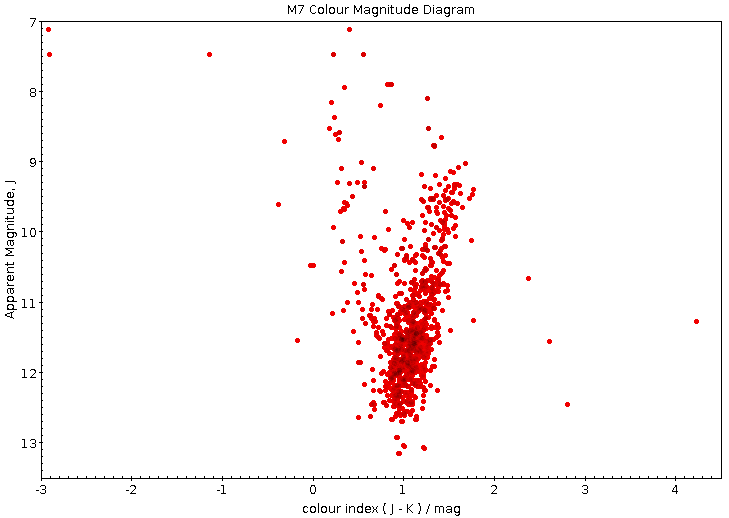
\includegraphics[width=\textwidth]{m7_cmd_apparent}
			\caption{M7 CMD plot using apparent magnitude}
			\label{fig: m7_cmd}
		\end{figure}
		\begin{figure}[h!]
			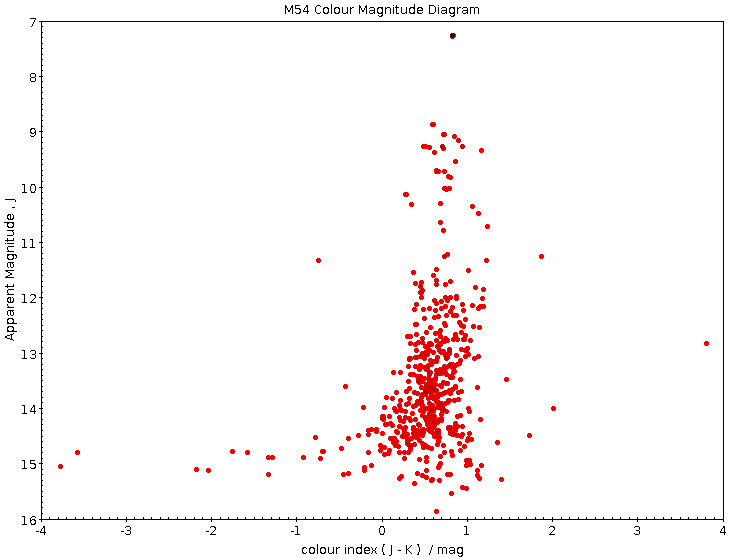
\includegraphics[width=\textwidth]{m54_cmd_apparent}
			\caption{M54 CMD plot using apparent magnitude}
			\label{fig: m54_cmd}
		\end{figure}
		\subsection{Applying for Corrections}
		We now account for physical effects that affect the shape of the CMD diagrams. The biggest effect is the \textbf{galactic extinction}. Galactic extinction refers to the effect of dust and gases in the Milky Way galaxy that causes the apparent magnitudes to be greater than they are i.e. it dims the light of objects within the galaxy and beyond the galaxy.\\
		Its effects are stronger at shorter wavelengths, resulting in starlight appearing redder than it normally is. This makes stars appear cooler. This shifts our J-K colour indices, hence our temperature estimates so that the stars are actually hotter than estimated (Danford \& Thomas 1981, Pandey et al.  2001).\\
		We thus have to apply an extinction correction. We make use of the NASA/IPAC Extragalactic Database (NED). We go to their tab on galactic extinctions to get the correction magnitudes. We use the UKIRT J and UKIRT K bandpasses. For M7, the galactic extinction magnitudes are 0.512 for UKIRT J and 0.218 for UKIRT K. For M54, these are 0.108 for UKIRT J and 0.046 for UKIRT K.\\
		The mathematical expression for the corrected magnitudes is as follows:
		\[M_{J, corrected} = M_{J, observed} - M_{Galactic \,\, Extinction}\]
		We will adjust our model by the galactic extinction and re-plot our CMD graphs.
		\begin{figure}
			\centering
			\subfloat[\centering M7 corrected CMD plot using corrected apparent magnitude]{{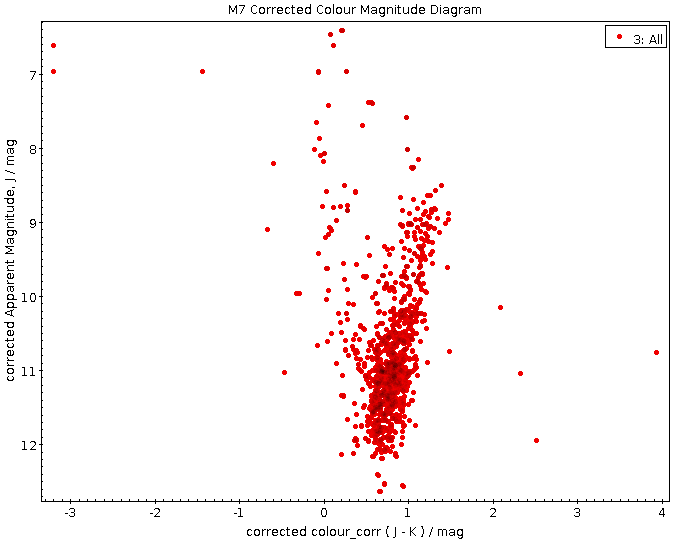
\includegraphics[width=0.7\textwidth, keepaspectratio]{m7_cmd_corrected_apparent}}}
			\qquad
			\subfloat[\centering M54 corrected CMD plot using corrected apparent magnitude]{{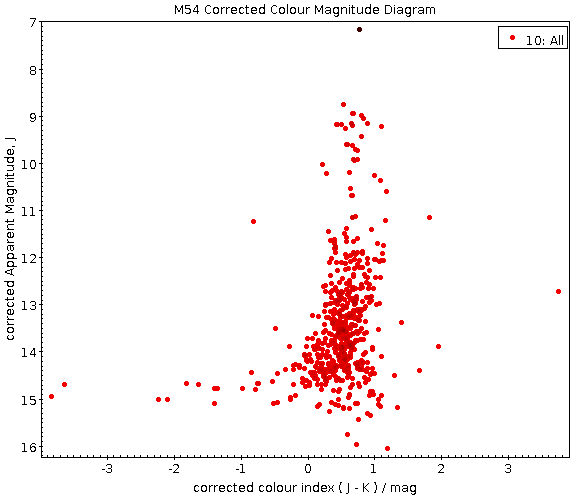
\includegraphics[width=0.7\textwidth, keepaspectratio]{m54_cmd_corrected_apparent}}}
			\caption{Extinction corrected CMD plots}
			\label{fig: m7_m54_cmd_corrected}
		\end{figure}
%		\begin{figure}
%			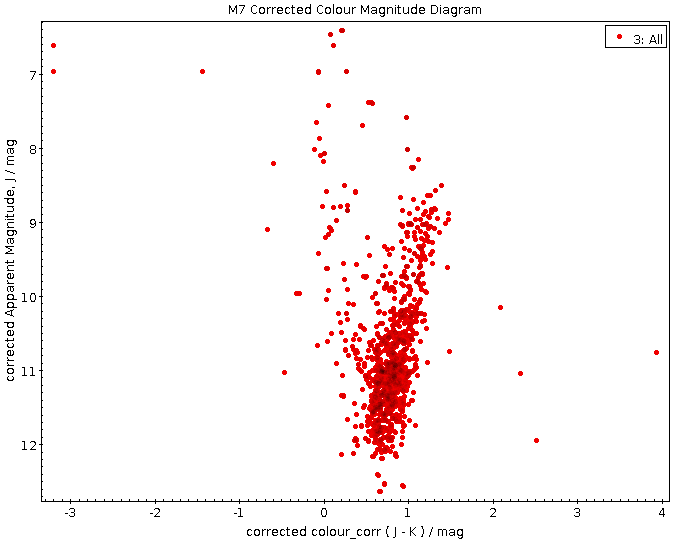
\includegraphics[width=\textwidth]{m7_cmd_corrected_apparent}
%			\caption{M7 corrected CMD plot using corrected apparent magnitude}
%			\label{fig: m7_cmd_corrected}
%		\end{figure}
%		\begin{figure}
%			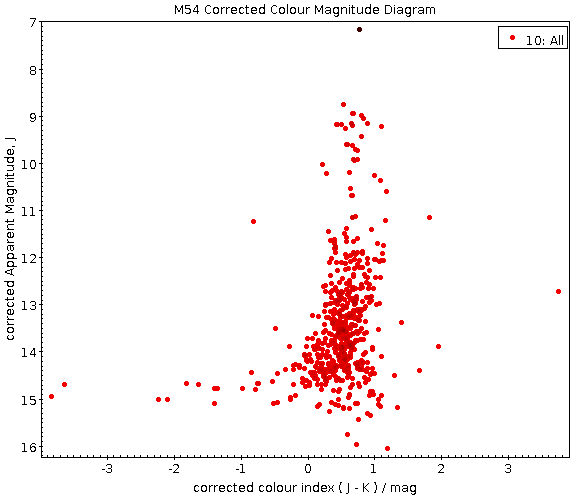
\includegraphics[width=\textwidth]{m54_cmd_corrected_apparent}
%			\caption{M54 corrected CMD plot using corrected apparent magnitude}
%			\label{fig: m54_cmd_corrected}
%		\end{figure}
		
		\subsection{Finding Age and Distance}
		Our approach into solving this process involves fitting a model isochrone. It is a fact that the absolute magnitudes of stars in different star clusters have some differences. However, using this method, we can fit a theoretical model of a cluster's stars to its Colour Magnitude Diagram. In this isochrone computer model, all stars have the same age, just as we would expect for clusters. In practice, the isochrone is a table os simulated stars, one star per row where the star columns give the star's absolute magnitude in different filters.\\
		Our resource website for getting our isochrones is \url{http://stev.oapd.inaf.it/cgi-bin/cmd}. It is a web interface dealing with stellar isochrones and their derivatives. We can download isochrones of different ages until and plot a fir for each one till we get a satisfactory fit that is closest to our CMD plot.\\
		We choose our photometric system as 2MASS JHKs. Next important section is the Ages/metallicities input information section. We will enter the desired age in initial value input box. Globular clusters tend to be old, thus we will use ages ranging from 1-14 Billion years. Since open clusters tend to be younger, our age ranges can be from 50-900 Million years.\\
		We choose 200e6 or 200 Million years for our M7 open cluster and 13e9 or 13 Billion years for our M54 globular cluster.\\
		Submit the input data and download the ASCII isochrone files.\\
		Load and open them up in TOPCAT. Open up their column metadata and de-select every column except the magnitude columns; in this case it is labelled Jmag and Ksmag. Note that the magnitude values for the J and K bands are absolute magnitudes, while our CMD uses apparent magnitudes.
		\subsubsection{Cluster Distance}
		When we overlay the two plots, i.e. the CMD and the isochrone plot, we observe a clear average difference in the plots. This is due to the difference in the absolute and apparent magnitudes. This difference is our \textbf{distance modulus}. The distance modulus is given by
		\[\text{distance modulus} \,\,\,\, m - M = 5\log_{10}(d) - 5\]
		Therefore, we can get our distance as
		\[d = 10^{\frac{m - M + 5}{5}}\]
		\begin{figure}
			\centering
			\subfloat[\centering M7 corrected CMD plot using corrected apparent magnitude overlayed against isochrone]{{	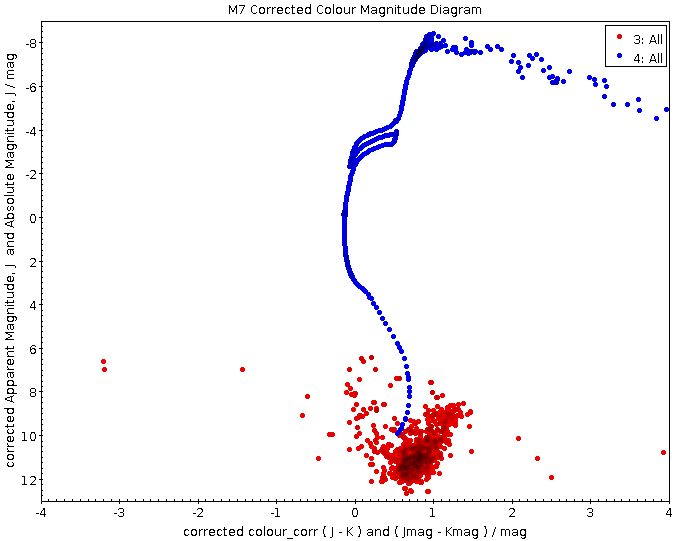
\includegraphics[width=0.7\textwidth, keepaspectratio]{m7_cmd_distance_modulus}}}
			\qquad
			\subfloat[\centering M54 corrected CMD plot using corrected apparent magnitude overlayed against isochrone]{{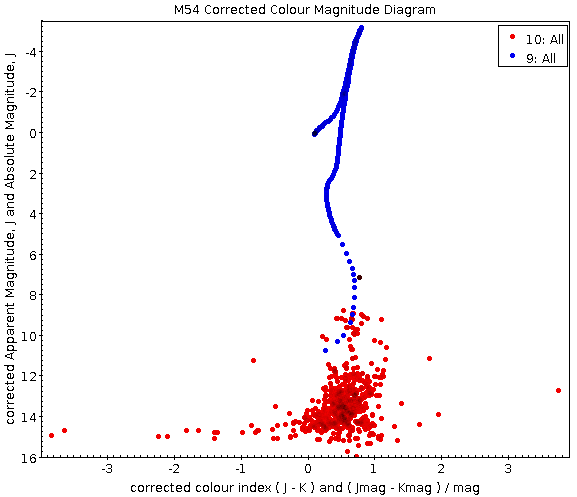
\includegraphics[width=0.7\textwidth, keepaspectratio]{m54_cmd_distance_modulus}}}
			\caption{Extinction corrected CMD plots overlayed against isochrone plots}
			\label{fig: m7_m54_distance_modulus}
		\end{figure}
%		\begin{figure}
%			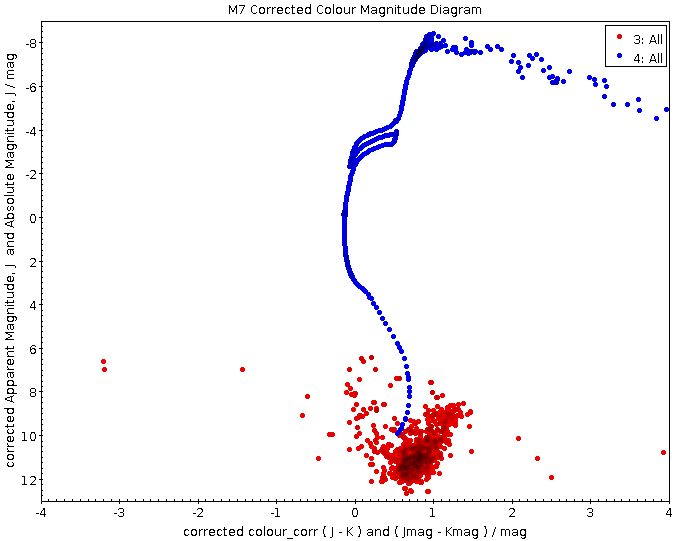
\includegraphics[width=0.5\textwidth, keepaspectratio]{m7_cmd_distance_modulus}
%			\caption{M7 corrected CMD plot using corrected apparent magnitude overlayed against isochrone}
%			\label{fig: m7_cmd_distance_modulus}
%		\end{figure}
%		\begin{figure}
%			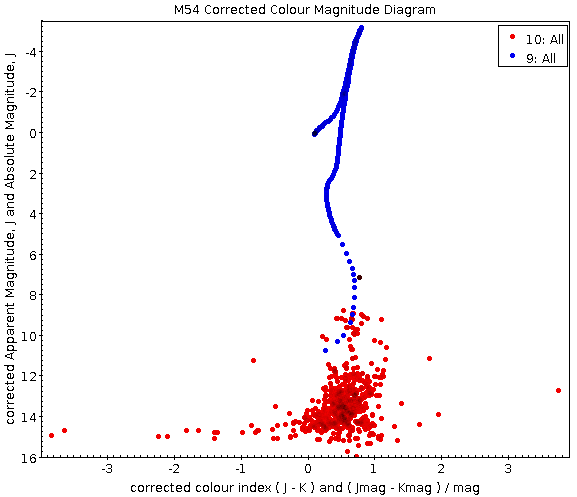
\includegraphics[width=0.5\textwidth, keepaspectratio]{m54_cmd_distance_modulus}
%			\caption{M54 corrected CMD plot using corrected apparent magnitude overlayed against isochrone}
%			\label{fig: m54_cmd_distance_modulus}
%		\end{figure}
		In order to scale down the isochrone plot, we will identify, from the overlayed plotting, the distance modulus i.e. the magnitude difference between the plots, and add it to the absolute magnitude value of the isochrone. This will give us the apparent magnitude of the isochrone.\[M_{isochrone} + (m_{apparent} - M_{isochrone}) = m_{apparent}\]
		Plotting the isochrone using the apparent magnitude aligns it with the rest of the CMD plot.\\
		For the open cluster M7, we find the distance modulus to be about 7.5. We can now use the distance formula as
		\[d = 10^{\frac{7.5 + 5}{5}} = \framebox{316.23 parsecs}\]
		This gives us an approximate distance to M7 as 316 parsecs.\\
		For the globular cluster M8, we find the distance modulus to be about 16.9. Using the distance formula
		\[d = 10^{\frac{16.9 + 5}{5}} = \framebox{23, 988.33 parsecs}\]
		The globular cluster M54 is approximately at a distance of 24Kpc.
		\begin{figure}
			\centering
			\subfloat[\centering M7 corrected CMD plot using corrected apparent magnitude overlayed against isochrone]{{	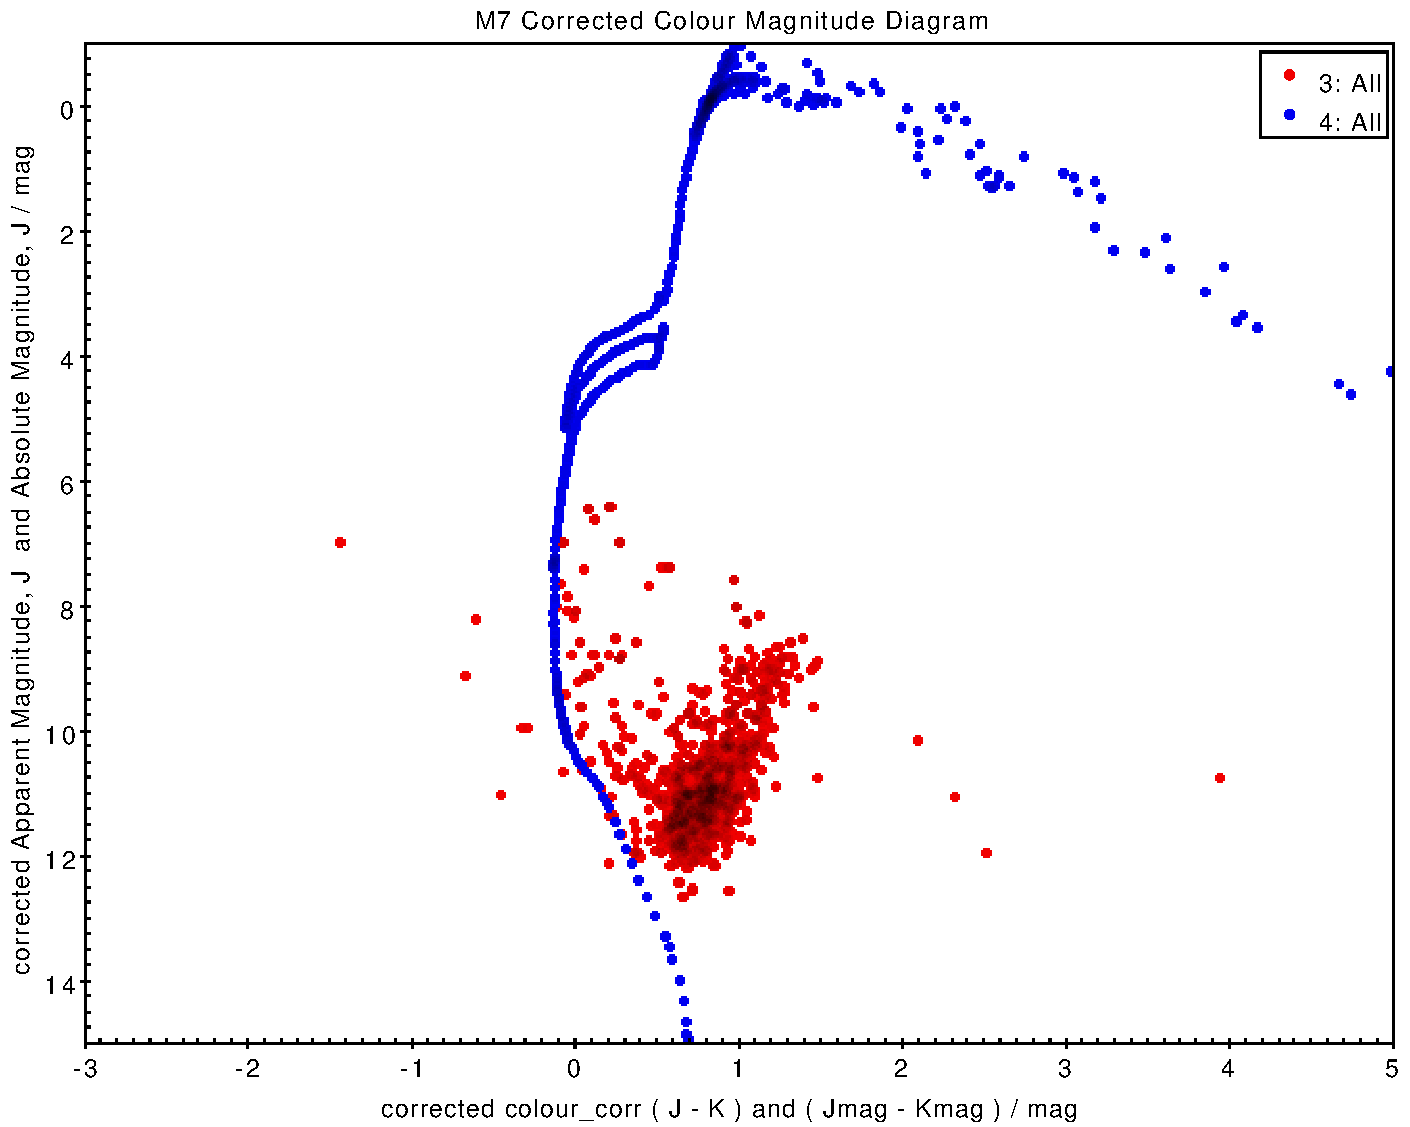
\includegraphics[width=0.7\textwidth, keepaspectratio]{m7_cmd_all}}}
			\qquad
			\subfloat[\centering M54 corrected CMD plot using corrected apparent magnitude overlayed against isochrone]{{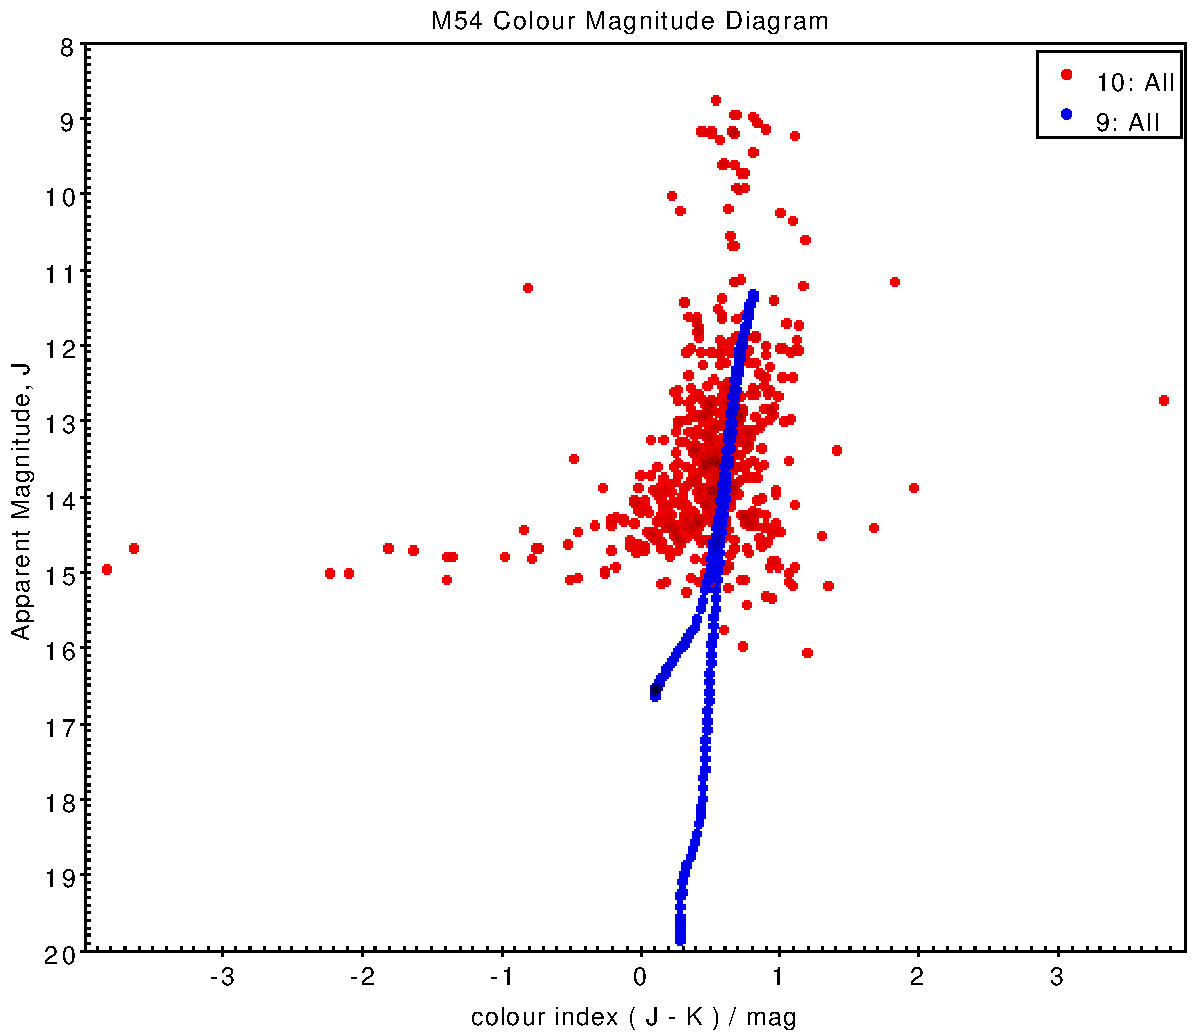
\includegraphics[width=0.7\textwidth, keepaspectratio]{m54_cmd_all}}}
			\caption{Extinction corrected CMD plots overlayed against isochrone plots with no distance modulus. Without distance modulus, the isochrone curves now use apparent magnitude and can fit in with the CMD plot.}
			\label{fig: m7_m54_all}
		\end{figure}
%		\begin{figure}
%			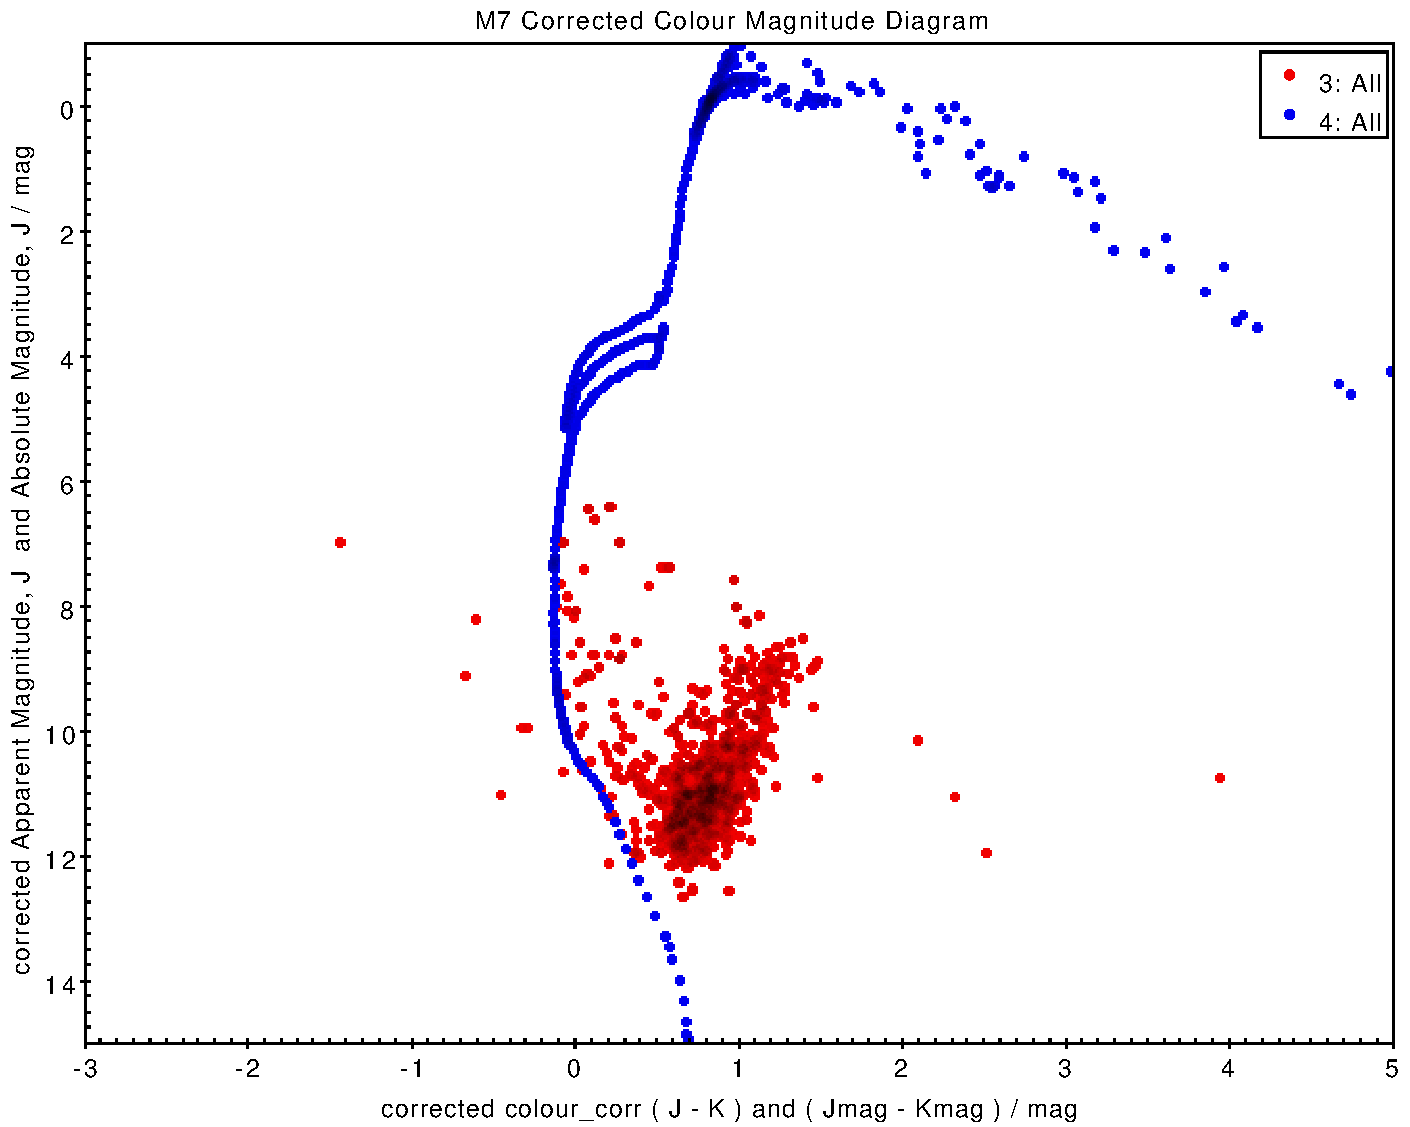
\includegraphics[scale=0.34]{m7_cmd_all}
%			\caption{M7 corrected CMD plot using corrected apparent magnitude overlayed against isochrone}
%			\label{fig: m7_cmd_all}
%		\end{figure}
%		\begin{figure}
%			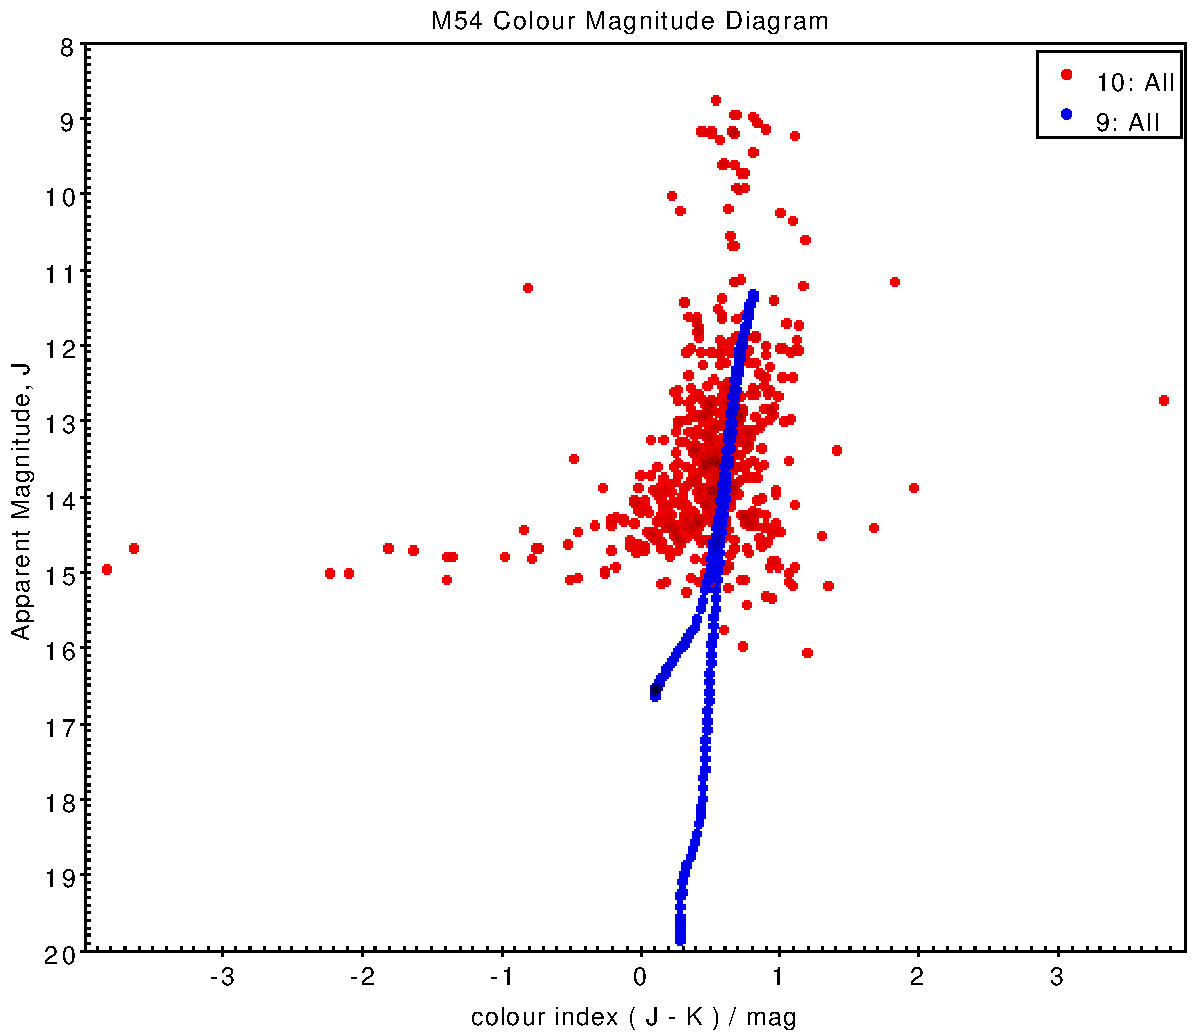
\includegraphics[scale=0.34]{m54_cmd_all}
%			\caption{M54 corrected CMD plot using corrected apparent magnitude overlayed against isochrone}
%			\label{fig: m54_cmd_all}
%		\end{figure}
		\pagebreak
		\subsubsection{Cluster Age}
		The age of a cluster is usually determined by the life expectancy of the most massive main sequence. We call this the \textbf{turnoff point}. Massive stars burn through their nuclear fuel much faster than their smaller main sequence counterparts.
		\begin{wrapfigure}{l}{0.60\textwidth}
			%\centering
			%\vspace{-30mm}
			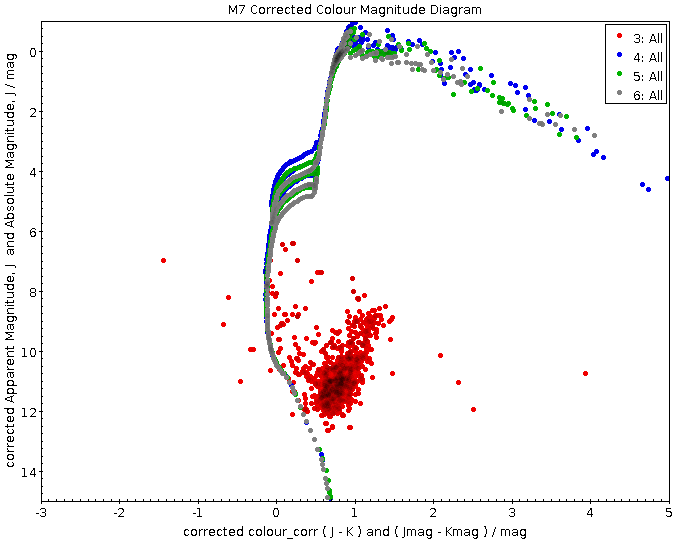
\includegraphics[width=0.58\textwidth, keepaspectratio]{m7_cmd_all_fits}
			\caption{3 isochrone overlays on CMD plot}
			\label{fig: m7_cmd_all_fits}
		\end{wrapfigure}
		It should come as no surprise then that the most massive star main sequence star in the cluster will be the first one to evolve off from the main sequence. Such a star also happens to be the most luminous of all main sequence star in the cluster.\\
		Normally on a HR diagram or CMD plot, this turnoff point appears as a bend in the otherwise linear shape of the main sequence.\\
		Overlaying the theoretical stellar evolution isochrones helps us determine the age of the cluster. The best choice fit isochrone for our CMD places both age and metallicity constraints on the stellar population. Using the downloaded isochrone data tables, we overlay as many as possible on our CMD to get a suitable fit as can be seen in the plot. The best for isochrone for the open cluster M7 had an age constraint of 200 Million years while for the M54 globular cluster, the age constraint was 13 Billion years.
		
	
	\section{Discussion}
	The colour of a star is usually determined by its surface temperature. Cooler stars are redder while mode blue stars are hotter. Stars in open clusters are typically young and their star's relatively small making them quite hot on the surface. Thus, on a HR or CMD diagram, many of these stars will appear on the blue parts of the spectrum.\\
	Stars in globular clusters are older and very large, making the stars have a cooler surface. On a HR or CMD diagram, they will mostly reside on the red parts of the spectrum.\\
	From our plots, we can see that the stars on the open cluster M7 have lower colour indices and are therefore more blue in colour.\\
	For our globular cluster M54, the stars cover a much larger range of colour indices but are mostly in the larger values of the colour indices.\\
		\subsection{Comparison with Archive Data}
		We compare results we got with our CMD analysis with that obtained by various researchers and published in archive databases. We compare with data obtained from WEBDA and NED.
		\subsubsection{M7 Data Comparison}
		We found that distance to M7 to be 316.23 parsecs.From WEBDA, the distance given is 301 parsecs. This is a very near accurate estimate.\\
		The age of M7 we found to be 200 Million years which is in close agreement to that given in the WEBDA database which is 220 Million years.
		\subsubsection{M54 Data Comparison}
		Our established distance to M54 we found to be 23, 988.33 parsecs. The NED website data gives an estimated distance of 26, 800 parsecs or 87, 400 light years.\\
		Our best isochrone fit for our CMD had an age of 13 Billion years; pretty much in accoradance with the NED website.
		\section{Conclusion}
		This work served as a proof of concept on how stellar cluster ages and distances can be determined from their luminosity. We observed measurements of ages and distances of two star clusters, the open cluster M7 and the globular cluster M54, based on stellar evolution calculations and isochrone fitting.\\
		Our method of age and distance works satisfactorily.\\
		Our overall conclusion is that studying star clusters using Colour Magnitude Diagrams and with appropriate theoretical methods of isochrone fitting can provide valuable new insights into stellar clusters as well as satisfactorily determine stellar distances and ages.
		
	\pagebreak
	\begin{thebibliography}{}
		
		\bibitem{albrecht}
		{Albrecht Uns\"{o}ld and Bodo Baschek},
		{The New Cosmos: An Introduction to Astronomy and Astrophysics},
		{Springer},{fifth edition}, 2001.
		
		\bibitem{bradley}
		{Bradely W. Carrol and Dale A. Ostlie},
		{An Introduction to Modern Astrophysics}
		{Pearson Education Limited},
		{second edition}, 2014.
		
		\bibitem{zeilik}
		{Michael Zeilik and Stephen A. Gregory},
		{Introductory Astronomy and Astrophysics},
		{Thomson Learning}, 1998.
		
		\bibitem{nasa_m54}
		{Hubble's Messier Catalog: Messier 54},
		{\url{https://www.nasa.gov/feature/goddard/2017/messier-54}},
		{[Last updated; Oct 19, 2017]},
		{[Online; accessed April 19, 2021]}
		
		\bibitem{messier54}
		{Messier Objects: Messier 54},
		{\url{https://www.messier-objects.com/messier-54/}},
		{[Last updated; June 10, 2015]},
		{[Online; accessed April 26, 2021]}
		
		\bibitem{messier007}
		{Messier 7: Ptolemy's Cluster},
		{\url{https://www.messier-objects.com/messier-7-ptolemys-cluster/}},
		{[Last updated; February 11, 2015]},
		{[Online; accessed April 16, 2021]}
		
		\bibitem{astropixels_m7}
		{M7 - Ptolemy Cluster},
		{\url{http://astropixels.com/openclusters/M7-01.html}},
		{[Last updated; 2011 June 28]},
		{[Online; accessed April 19, 2021]}
		
		\bibitem{esahubble_images}
		{Image Archive: Star Clusters},
		{\url{https://esahubble.org/images/archive/category/starclusters/}},
		{[Online; accessed April 19, 2021]}
		
		\bibitem{eso_m7}
		{The star cluster Messier 7},
		{\url{https://www.eso.org/public/images/eso1406a/}},
		{[Online; accessed April 19, 2021]}
		{[Release date: 19 February 2014, 12:00]}
		
		\bibitem{eso_m54}
		{The globular star cluster Messier 54},
		{\url{https://www.eso.org/public/images/eso1428a/}},
		{[Online: accessed April 19, 2021]}
		{[Release date: 10 September 2014, 12:00]}
		
	\end{thebibliography}


\end{document}